% Files using this must be two subfolders
% deep. Adjust the number of ../ for the
% depth of the file.
% Imports
\usepackage{fancyhdr}
\usepackage{geometry}
\usepackage{icomma}
\usepackage{amsmath}
\usepackage{multicol}
\usepackage{mathptmx}
\usepackage{anyfontsize}
\usepackage{t1enc}
\usepackage{tabto}
\usepackage{listings}
\usepackage{filecontents}
\usepackage{subcaption}
\usepackage{tikz}
\usepackage[parfill]{parskip}
\usepackage{graphicx}
\usepackage[]{mdframed}
\usepackage{amsmath}
\usepackage[makeroom]{cancel}
\usepackage{pgfplots}
\usepackage{pgfplotstable}
\usepackage{xfrac}
\usepackage{amssymb}
\usepackage{mathtools}
\pgfplotsset{compat=1.18}
\usetikzlibrary{patterns}
\usepgfplotslibrary{polar}
\usepgfplotslibrary{fillbetween}

\geometry{margin=2.5cm}

\newcommand{\name}{Kaleb Burris}
\newcommand{\classname}{MATH F253, Elizabeth S. Allman, University of Alaska Fairbanks}
\newcommand{\assignment}{FILL IN ASSIGNMENT NAME}

\pagestyle{fancy}

\fancyhead[L]{
    \name 
    \newline
    \classname
    \newline
    \assignment
}

\newcommand{\horizontal}{\noindent\rule{\hsize}{0.4pt}}

\setlength{\headheight}{42pt}
\setlength{\headsep}{0.25in}
\setlength{\columnsep}{0.35cm}
\setlength{\columnseprule}{1pt}

\usepackage[T1]{fontenc}
\usepackage{lmodern}

\usepackage{graphicx}
\graphicspath{ {./lab01images/} }

% Put class number, class name, and professor 
% name.
% Use only in case of emergency, this
% should be covered by the preamble.
% \renewcommand\classname{}

% Put the assignment name with \S if 
% necessary for the section and the question 
% numbers.
\renewcommand\assignment{Lab 1: Distance, Velocity, Acceleration, 1/31/2023, Partners: Maite Valentin-Lugo, Seth Waln}

\begin{document}

    % Templates
    \iffalse
    % Use these for equations.
    \begin{equation*}
        \begin{gathered}
            Equations go here.
        \end{gathered}
    \end{equation*}

    % Use this if a line of math is too long.
    \resizebox{\hsize}{!}{$Long equation goes here$}

    % Use these for multiple columns.
    \begin{multicol*}{# of columns}
        % Remove the * if you want the columns to be balanced.
    \end{multicol*}

    % Use this to add a horizontal line.
    \horizontal

    \fi

    % Begin homework here.
    %%%%%%%%%%%%%%%%%%%%%%

    \section*{Lab 1: Distance, Velocity, Acceleration}

    \subsection*{Apparatus}

    \begin{itemize}
        \item Motion detector
        \item Vernier LabQuest
        \item Logger Pro software
        \item Cart
        \item Basketball
        \item Foam Board
        \item Meter stick
        \item Colored pencils
    \end{itemize}

    \subsection*{Objective}

    \begin{itemize}
        \item Examine the relationship between distance, velocity and acceleration
        \item Attempt to duplicate given graphs with your own body's motion, or by moving a cart back and forth, quantitatively
        \item Consider what positive and negative values mean when applied to distance, velocity, and acceleration measurements
        
    \end{itemize}

    \subsection*{Part I: Distance vs Time}

    \subsection*{1.}
    Predict a distance vs time plot for slow, steady constant motion away from the detector.

    \begin{mdframed}
        \centering\begin{tikzpicture}[scale=1.25]
            \begin{axis}[
                axis lines=middle,
                axis line style={->},
                x label style={at={(axis description cs:0.5,-0.1)},anchor=north},
                y label style={at={(axis description cs:-0.1,.5)},rotate=90,anchor=south},
                xlabel={time (s)},
                ylabel={position (m)},
                axis equal
            ]
            \addplot[red, samples=100, domain=0:5]{x};
            \end{axis}
        \end{tikzpicture}
    \end{mdframed}

    \subsection*{2.}
    Now test your prediction: Collect data for slow, steady motion away from the detector. When you click the “Collect” button (Logger Pro) it will collect and plot data for 10 seconds. Either walk back and forth with the foam board or move the cart back and forth in front of the motion detector.

    \begin{mdframed}
        \centering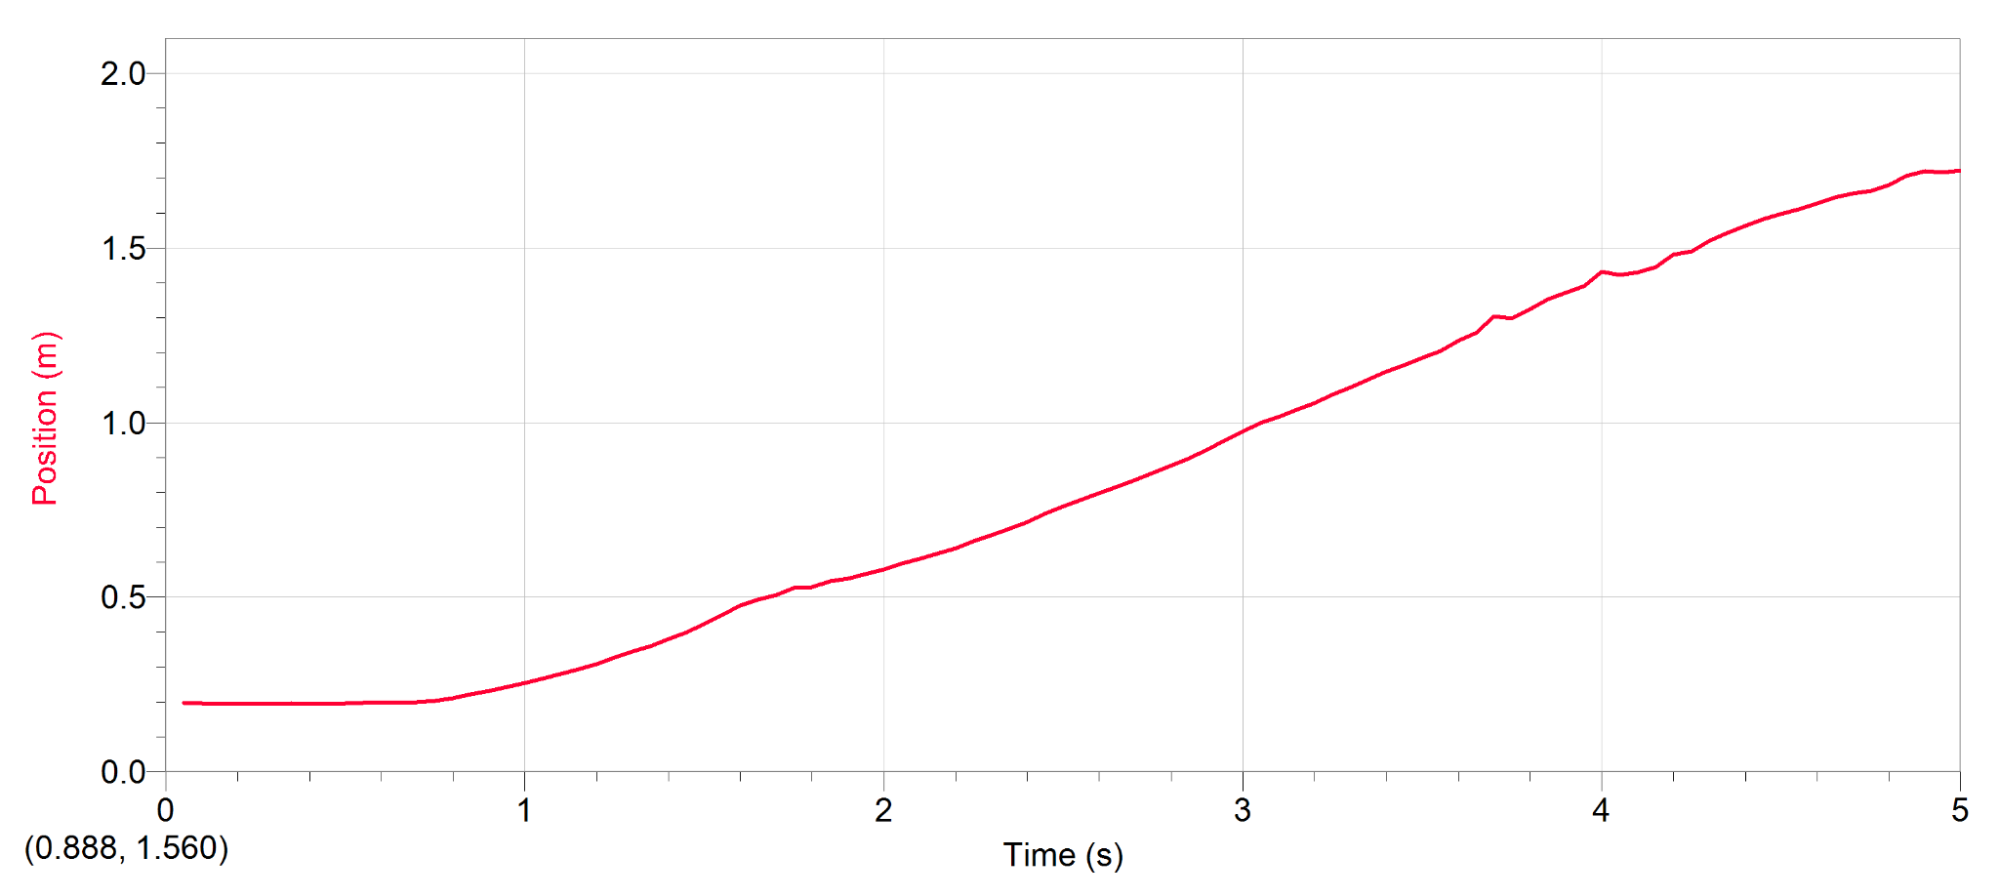
\includegraphics[width=0.5\textwidth]{image23.png}
    \end{mdframed}

    \subsection*{3.}
    Predict a distance vs time plot for slow, steady constant motion toward the detector.

    \begin{mdframed}
        \centering\begin{tikzpicture}[scale=1.5]
            \begin{axis}[
                axis lines=middle,
                axis line style={->},
                x label style={at={(axis description cs:0.5,-0.1)},anchor=north},
                y label style={at={(axis description cs:-0.1,.5)},rotate=90,anchor=south},
                xlabel={time (s)},
                ylabel={position (m)},
                axis equal,
                ymin=0,ymax=2,
                xmin=0,xmax=5
            ]
            \addplot[red, samples=100]{2-(2/5)*x};
            \end{axis}
        \end{tikzpicture}
    \end{mdframed}

    \pagebreak

    \subsection*{4.}
    Test your prediction: Collect data for slow, steady motion toward the detector. 

    \begin{mdframed}
        \centering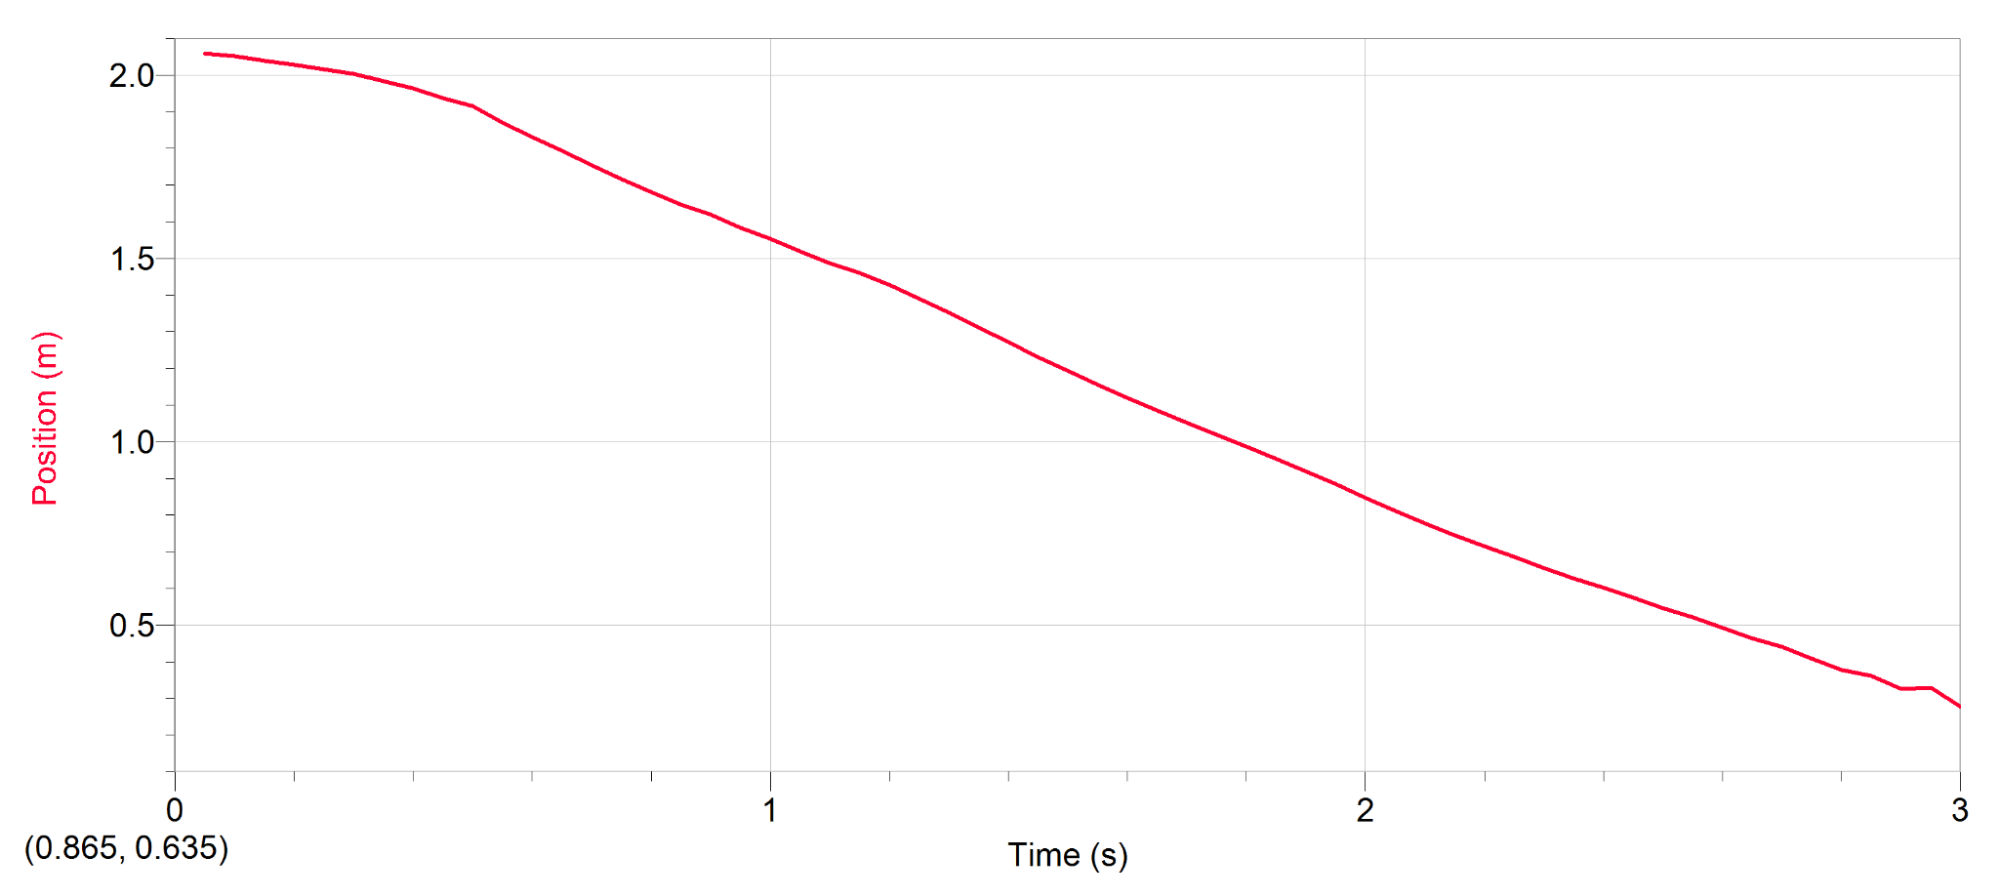
\includegraphics[width=0.8\textwidth]{image11.png}
    \end{mdframed}

    \subsection*{5.}
    Predict a distance vs. time plot for fast steady motion away from the detector (not speeding up, but faster than last time).

    \begin{mdframed}
        \centering\begin{tikzpicture}[scale=1.5]
            \begin{axis}[
                axis lines=middle,
                axis line style={->},
                x label style={at={(axis description cs:0.5,-0.1)},anchor=north},
                y label style={at={(axis description cs:-0.1,.5)},rotate=90,anchor=south},
                xlabel={time (s)},
                ylabel={position (m)},
                axis equal,
                ymin=0,ymax=5,
                xmin=0,xmax=2
            ]
            \addplot[red, samples=100]{3*x};
            \end{axis}
        \end{tikzpicture}
    \end{mdframed}

    \pagebreak

    \subsection*{6.}
    Test your prediction: Collect data for fast, steady motion away from the detector. 

    \begin{mdframed}
        \centering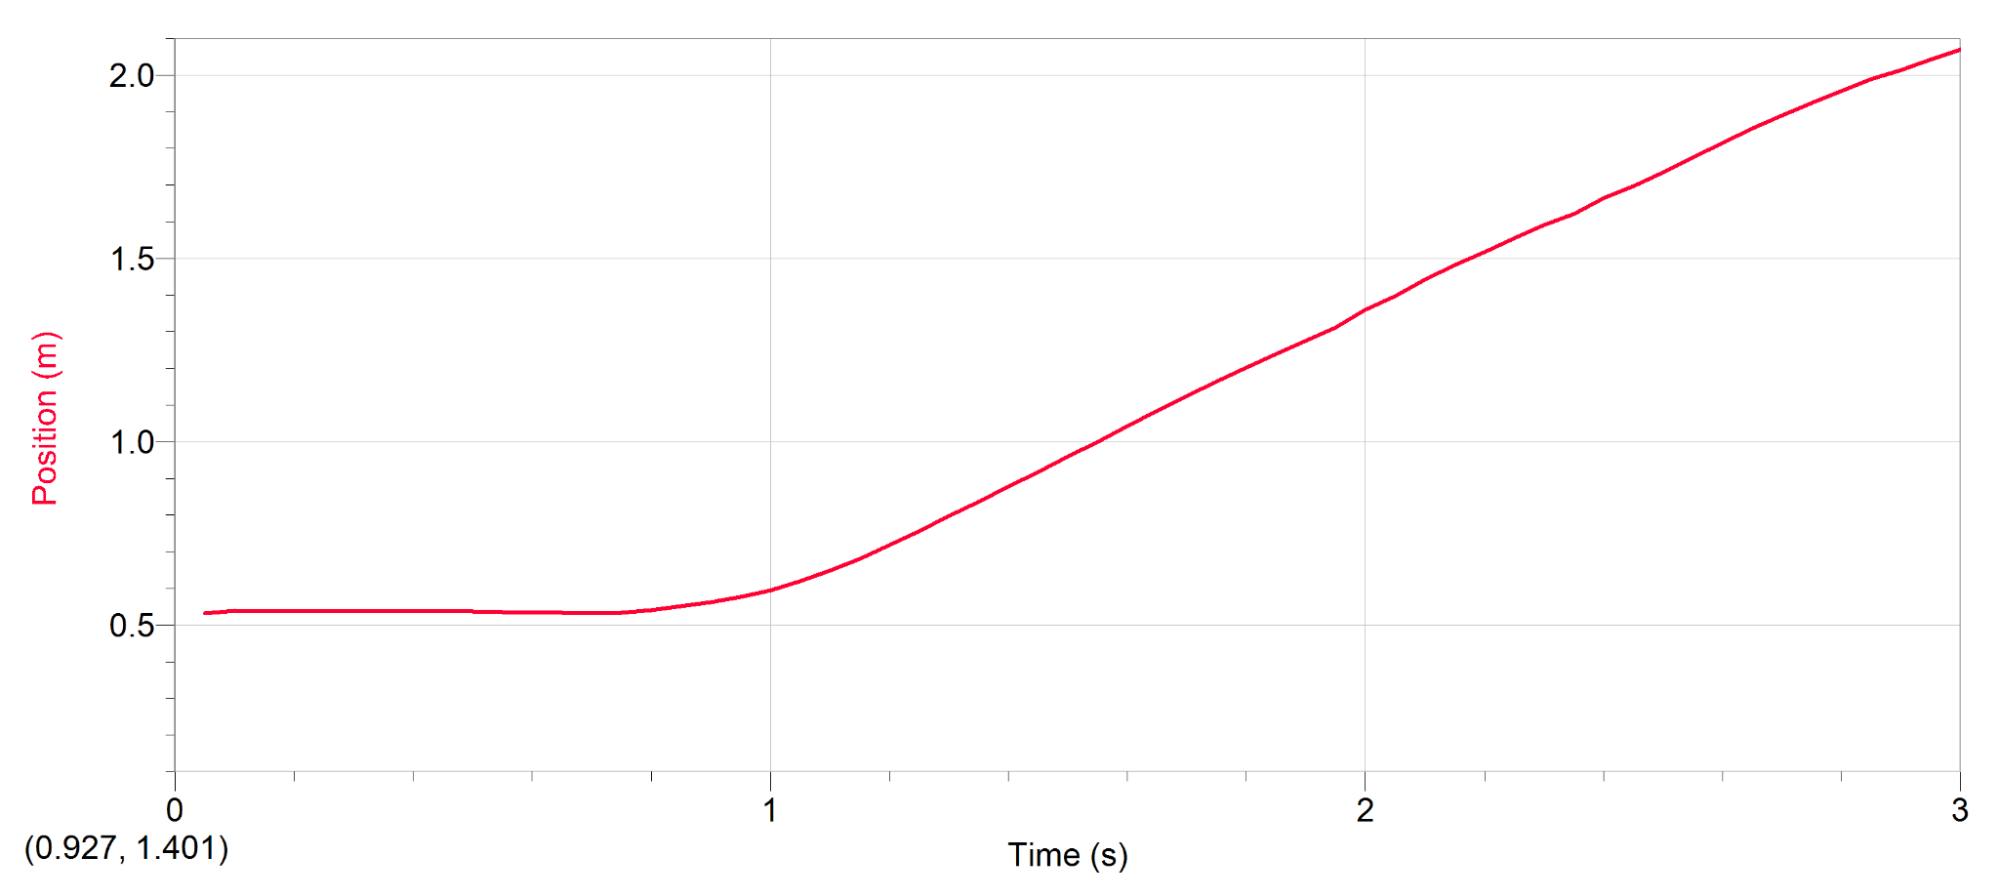
\includegraphics[width=0.8\textwidth]{image4.png}
    \end{mdframed}

    \subsection*{7,8.}
    Predict, then collect data for fast steady motion toward the detector.

    \begin{mdframed}
        \centering Prediction:

        \begin{tikzpicture}[scale=1.5]
            \begin{axis}[
                axis lines=middle,
                axis line style={->},
                x label style={at={(axis description cs:0.5,-0.1)},anchor=north},
                y label style={at={(axis description cs:-0.1,.5)},rotate=90,anchor=south},
                xlabel={time (s)},
                ylabel={position (m)},
                axis equal,
                ymin=0,ymax=2,
                xmin=0,xmax=4
            ]
            \addplot[red, samples=100]{2-(1/2)*x};
                
            \end{axis}
        \end{tikzpicture}

        Results:

        \centering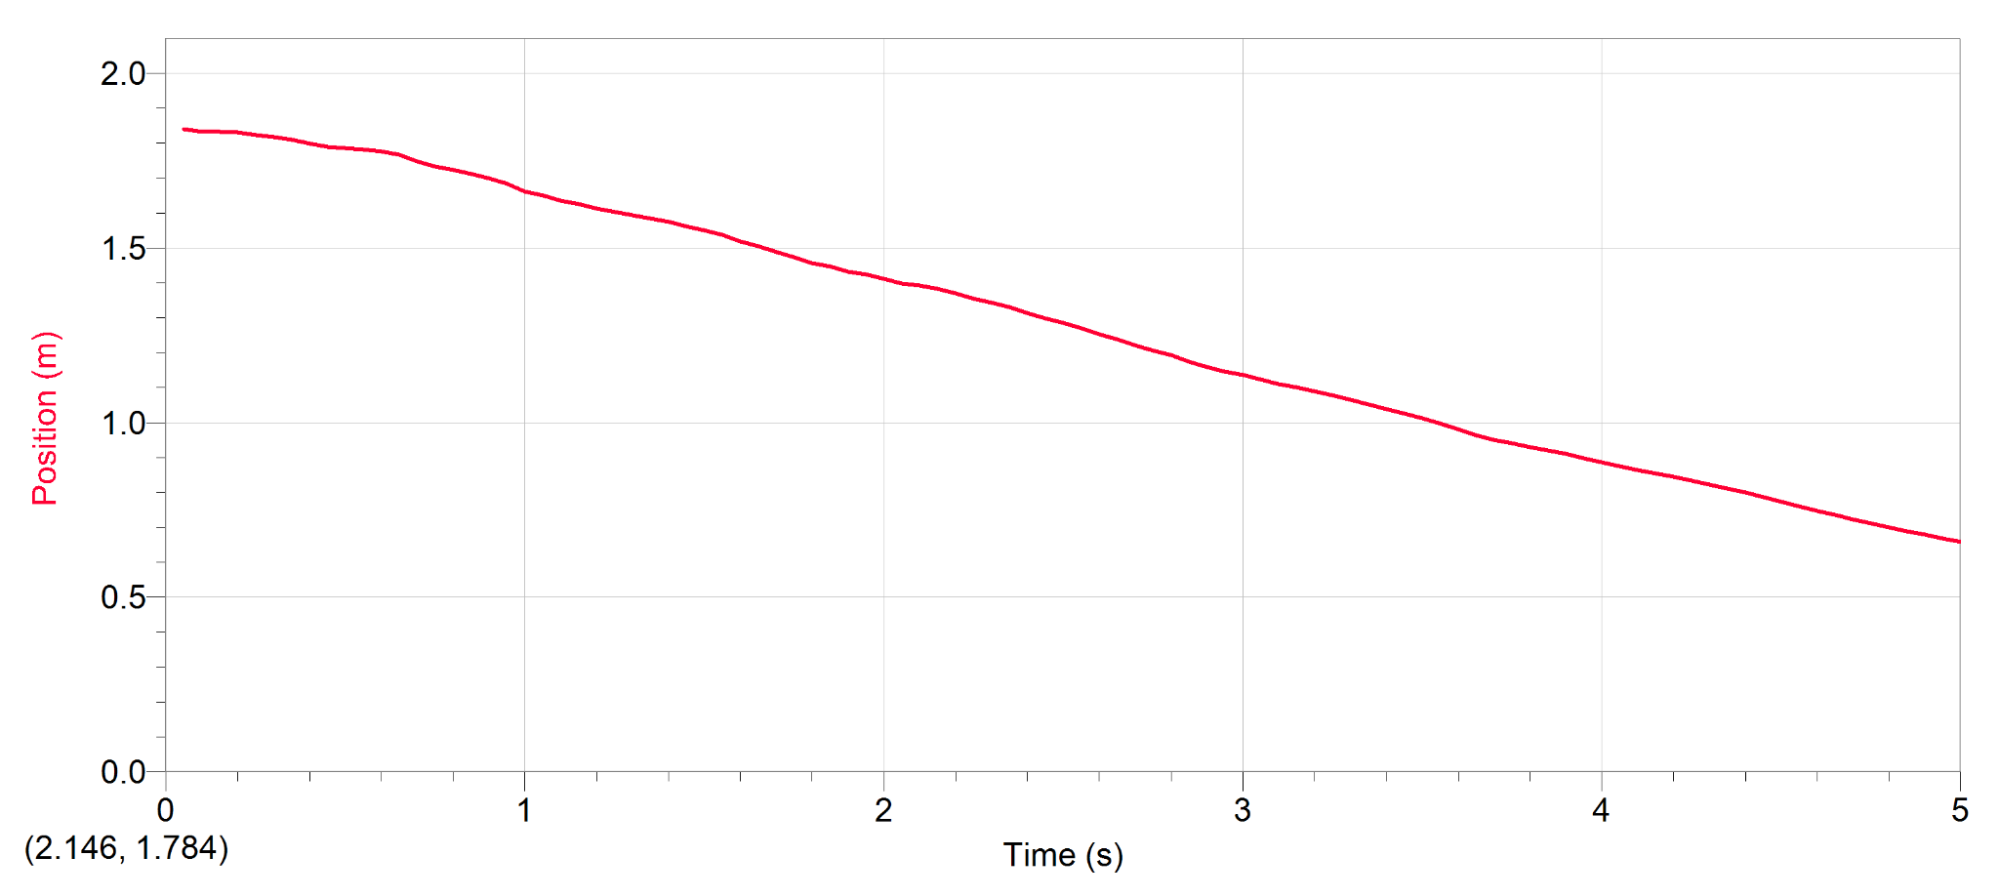
\includegraphics[width=0.8\textwidth]{image20.png}
    \end{mdframed}

    \subsection*{9.}
    Summarize the results of your observations using words such as: moving towards, moving away, fast, slow, positive slope, negative slope, steep, less steep.

    \begin{mdframed}
        
    \end{mdframed}

    \section*{Part II}

    \subsection*{10.}
    Predict a velocity vs time plot for slow, steady constant motion away from the detector. 

    \begin{mdframed}
        
    \end{mdframed}

    \subsection*{11.}
    Now test your prediction: Collect data for slow, steady motion away from the detector.

    \begin{mdframed}
        \centering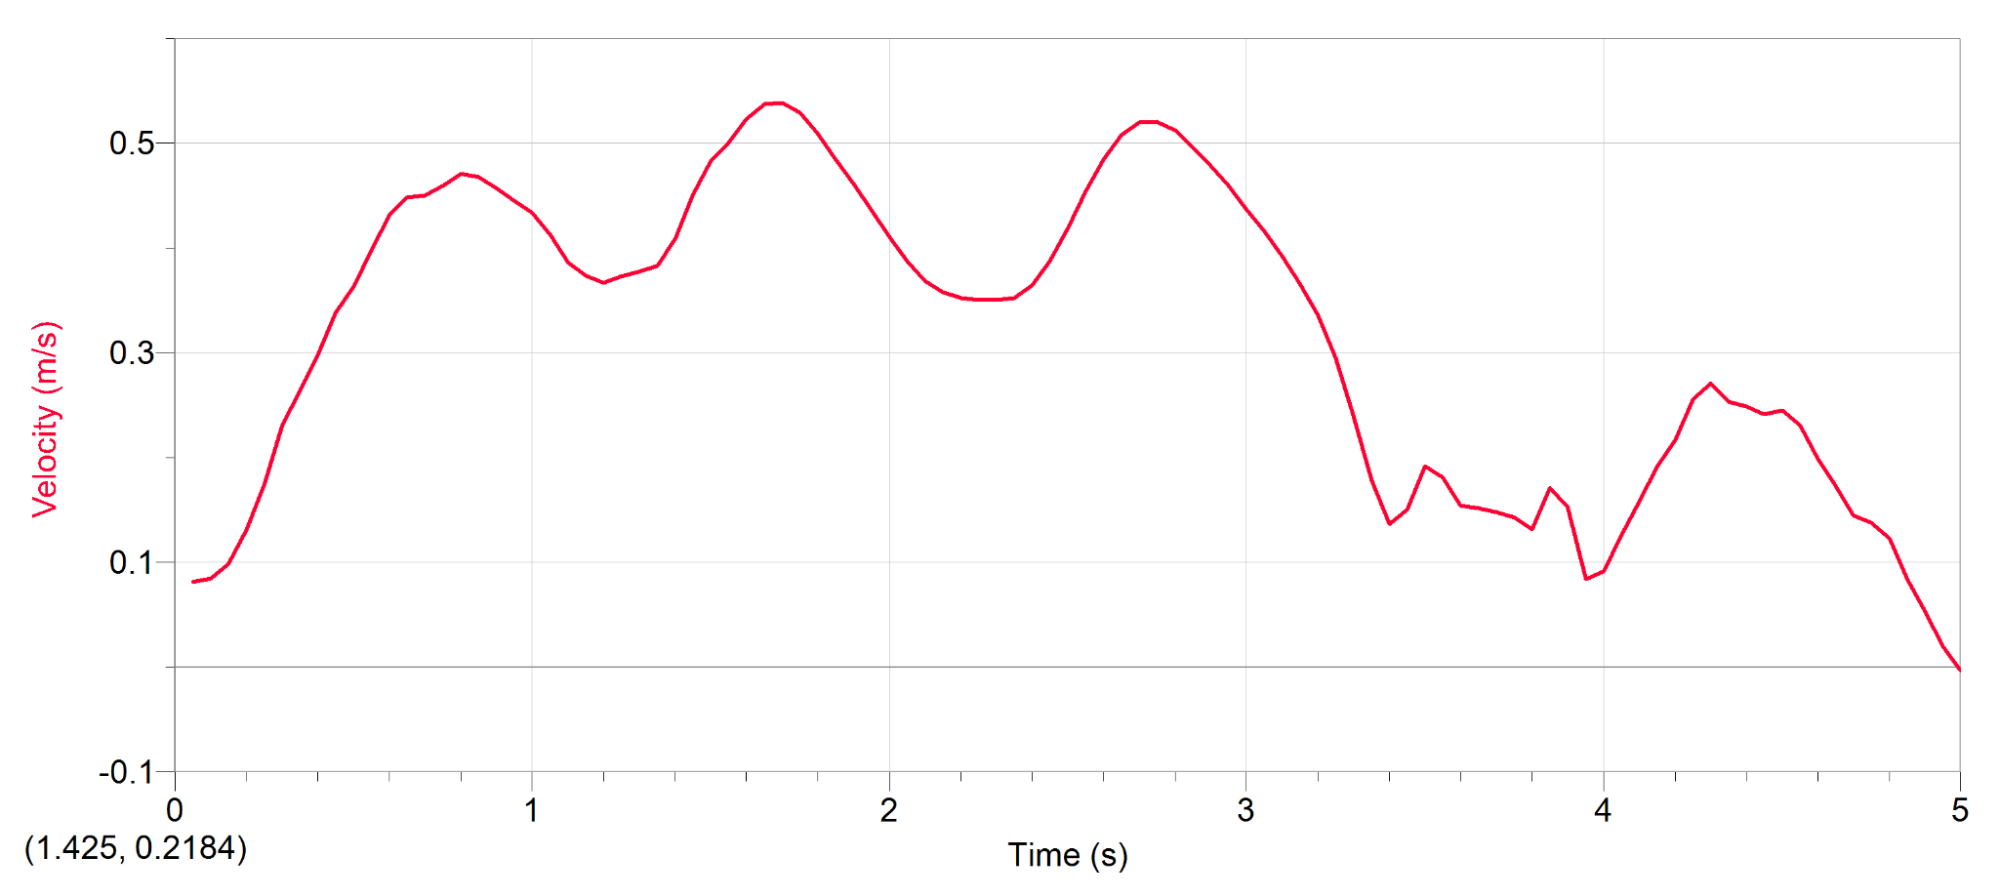
\includegraphics[width=0.8\textwidth]{image5.png}
    \end{mdframed}

    \subsection*{12.}
    Predict a velocity vs time plot for slow, steady constant motion toward from the detector. 

    \begin{mdframed}
        
    \end{mdframed}

    \subsection*{13.}
    Now test your prediction: Collect data for slow, steady motion toward from the detector.

    \begin{mdframed}
        \centering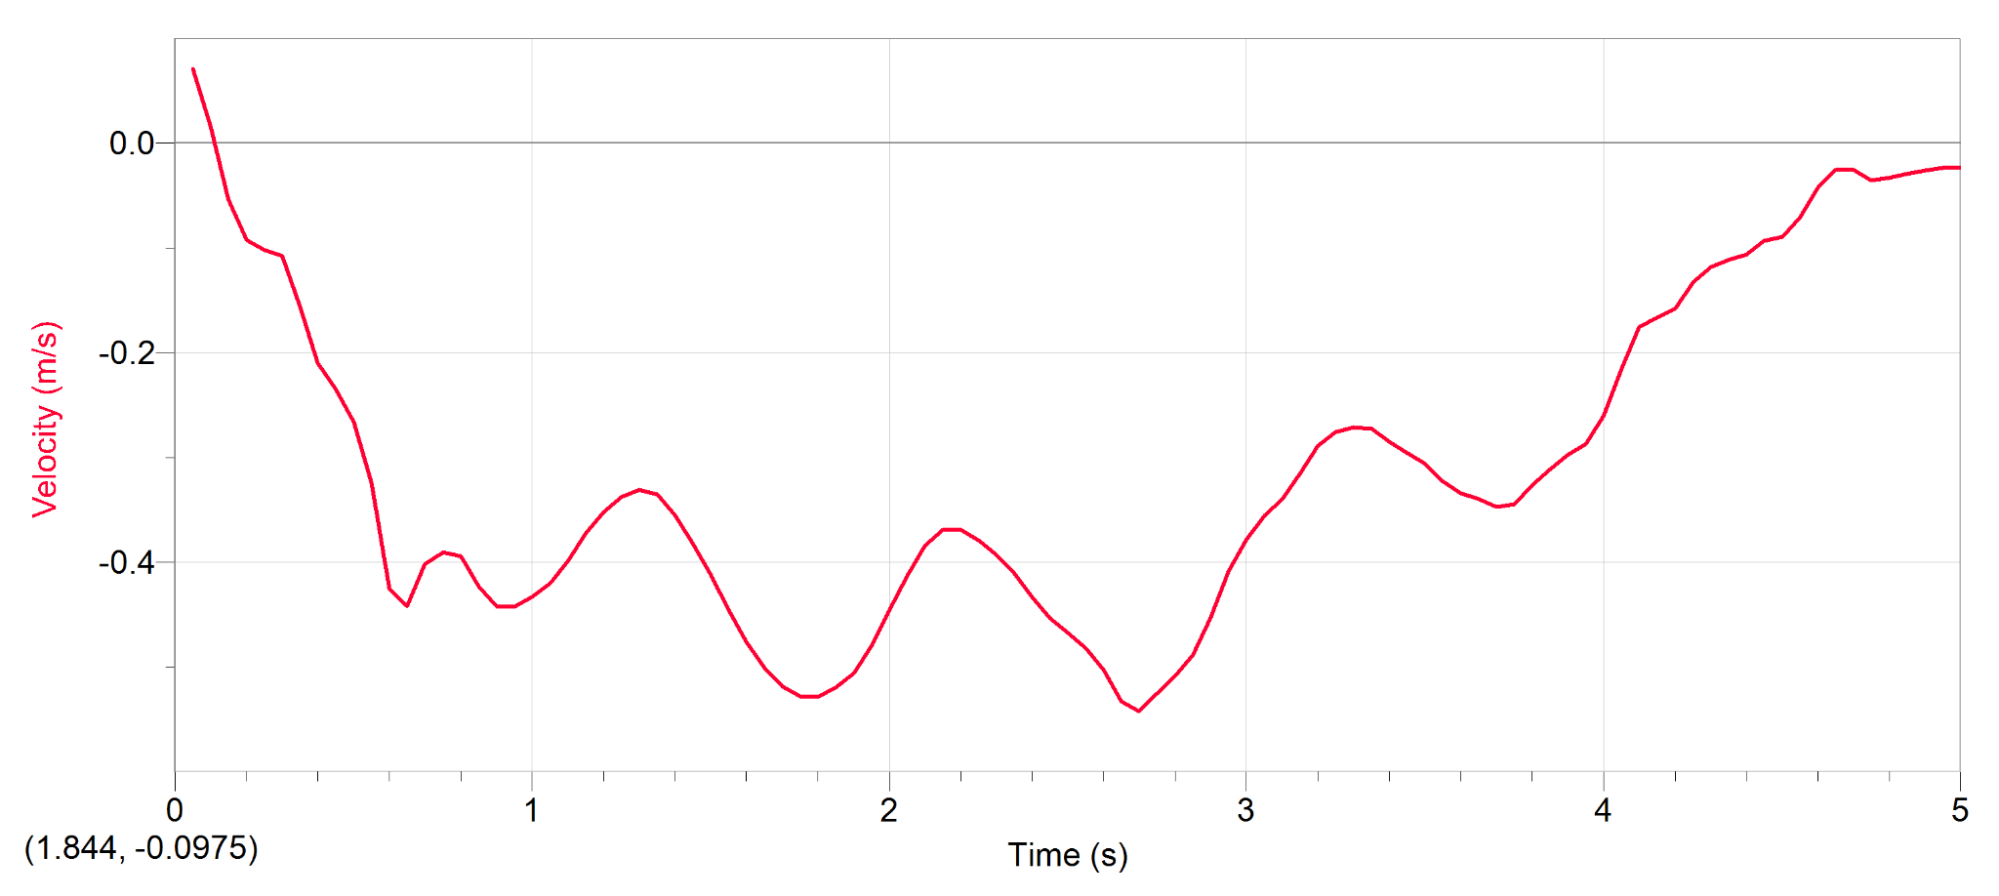
\includegraphics[width=0.8\textwidth]{image6.png}
    \end{mdframed}


    \subsection*{14.}
    Predict a velocity vs time plot for fast, steady constant motion away from the detector. 

    \begin{mdframed}
        
    \end{mdframed}

    \subsection*{15.}
    Now test your prediction: Collect data for fast, steady motion away from the detector.

    \begin{mdframed}
        \centering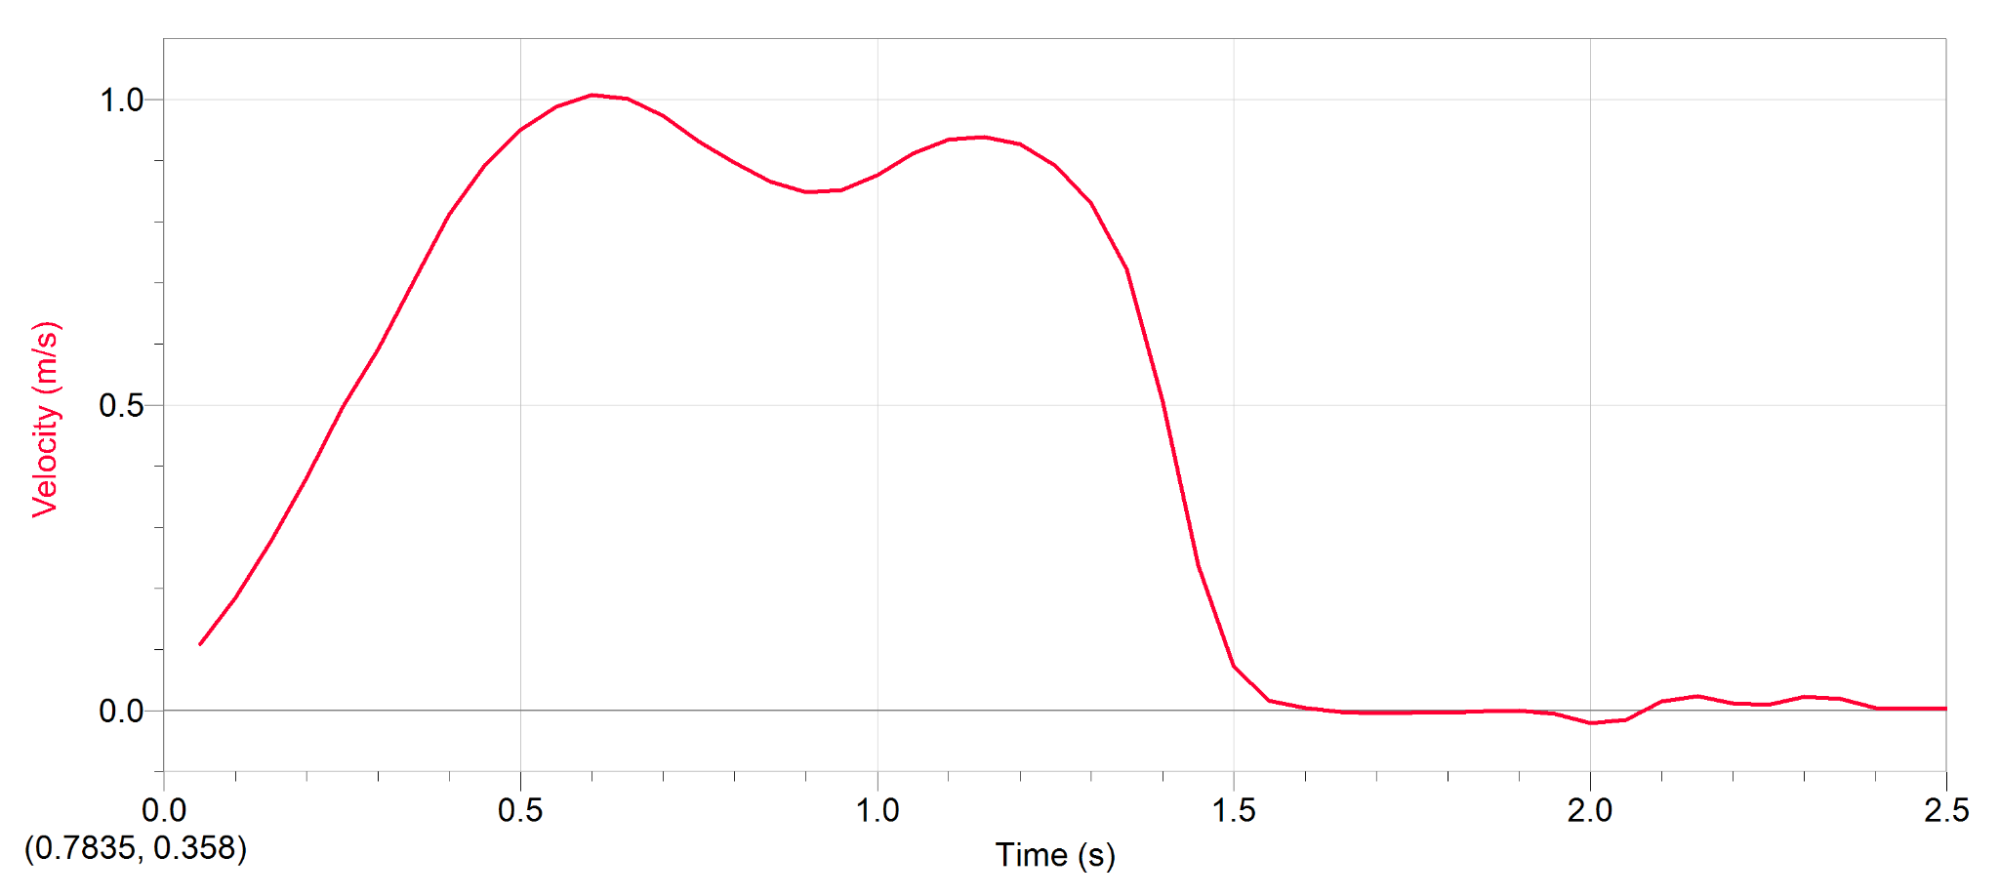
\includegraphics[width=0.8\textwidth]{image12.png}
    \end{mdframed}

    \subsection*{16.}
    Predict a velocity vs time plot for fast, steady constant motion away from the detector. 

    \begin{mdframed}
        
    \end{mdframed}

    \subsection*{17.}
    Now test your prediction: Collect data for fast, steady motion away from the detector.

    \begin{mdframed}
        \centering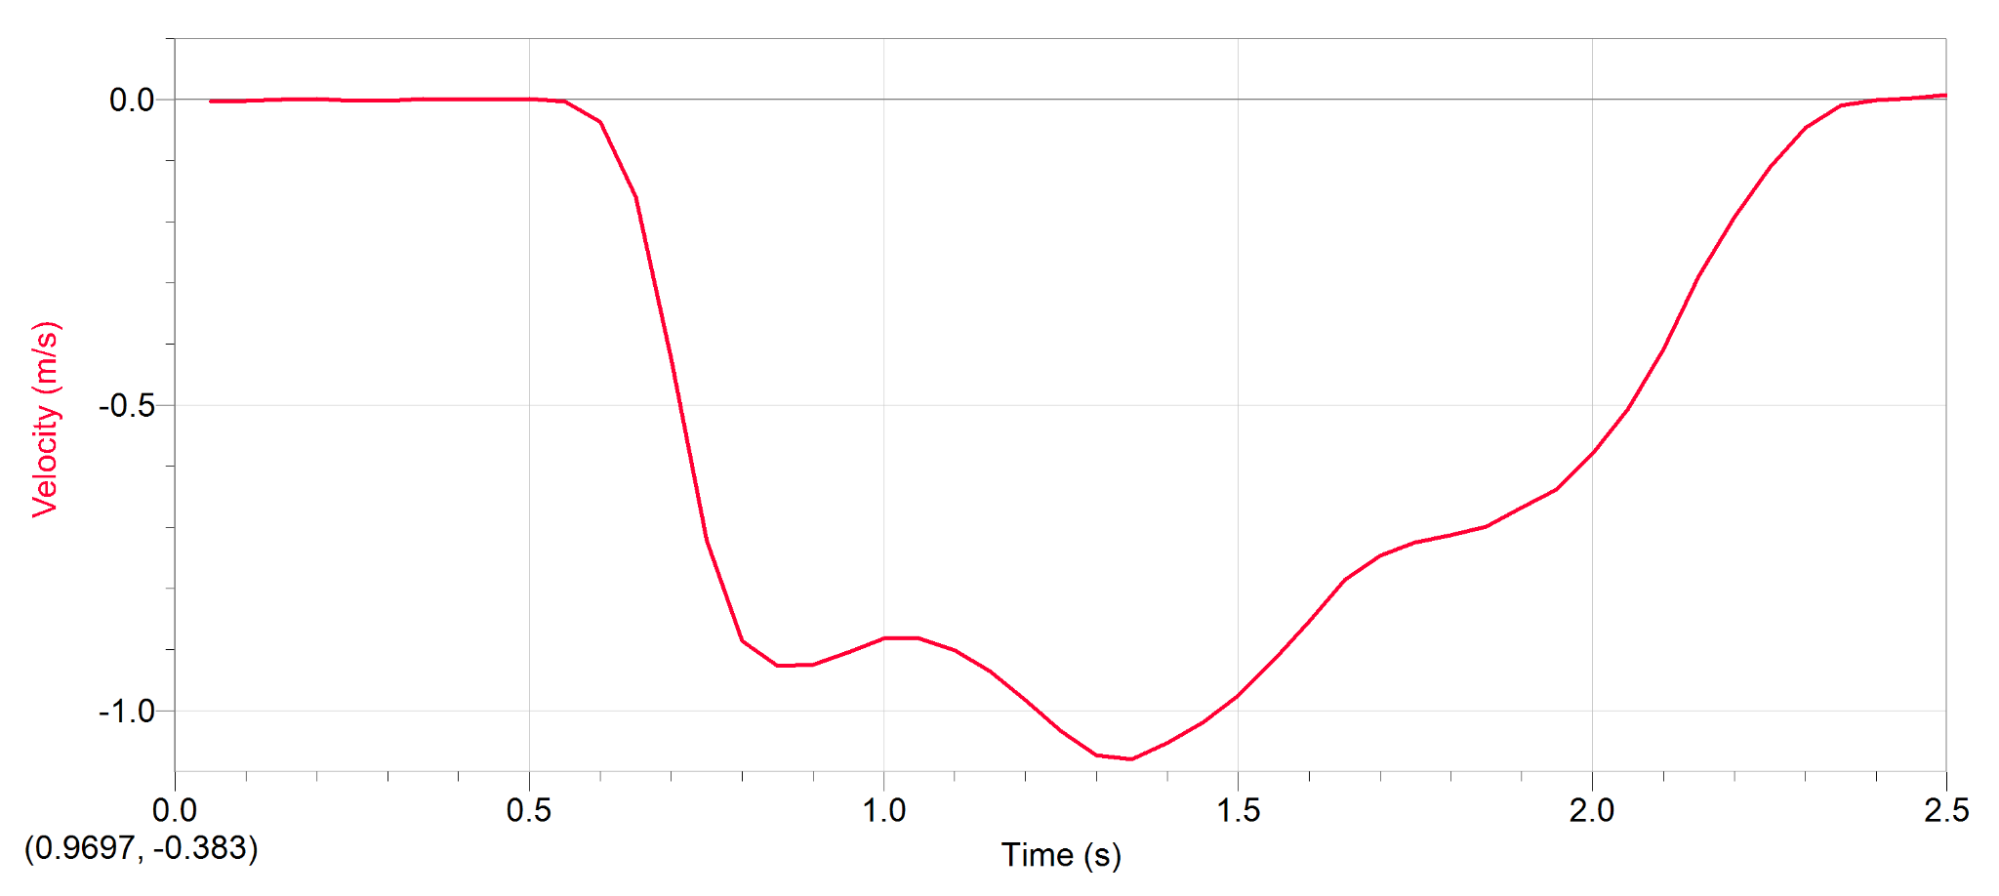
\includegraphics[width=0.8\textwidth]{image21.png}
    \end{mdframed}

    \subsection*{18.}
    Summarize the results of your observations using words such as: moving towards, moving away, fast, slow, positive value, negative value, far from the time axis, close to the time axis.

    \section*{Part III}

    \subsection*{19.}

    \begin{mdframed}
        \centering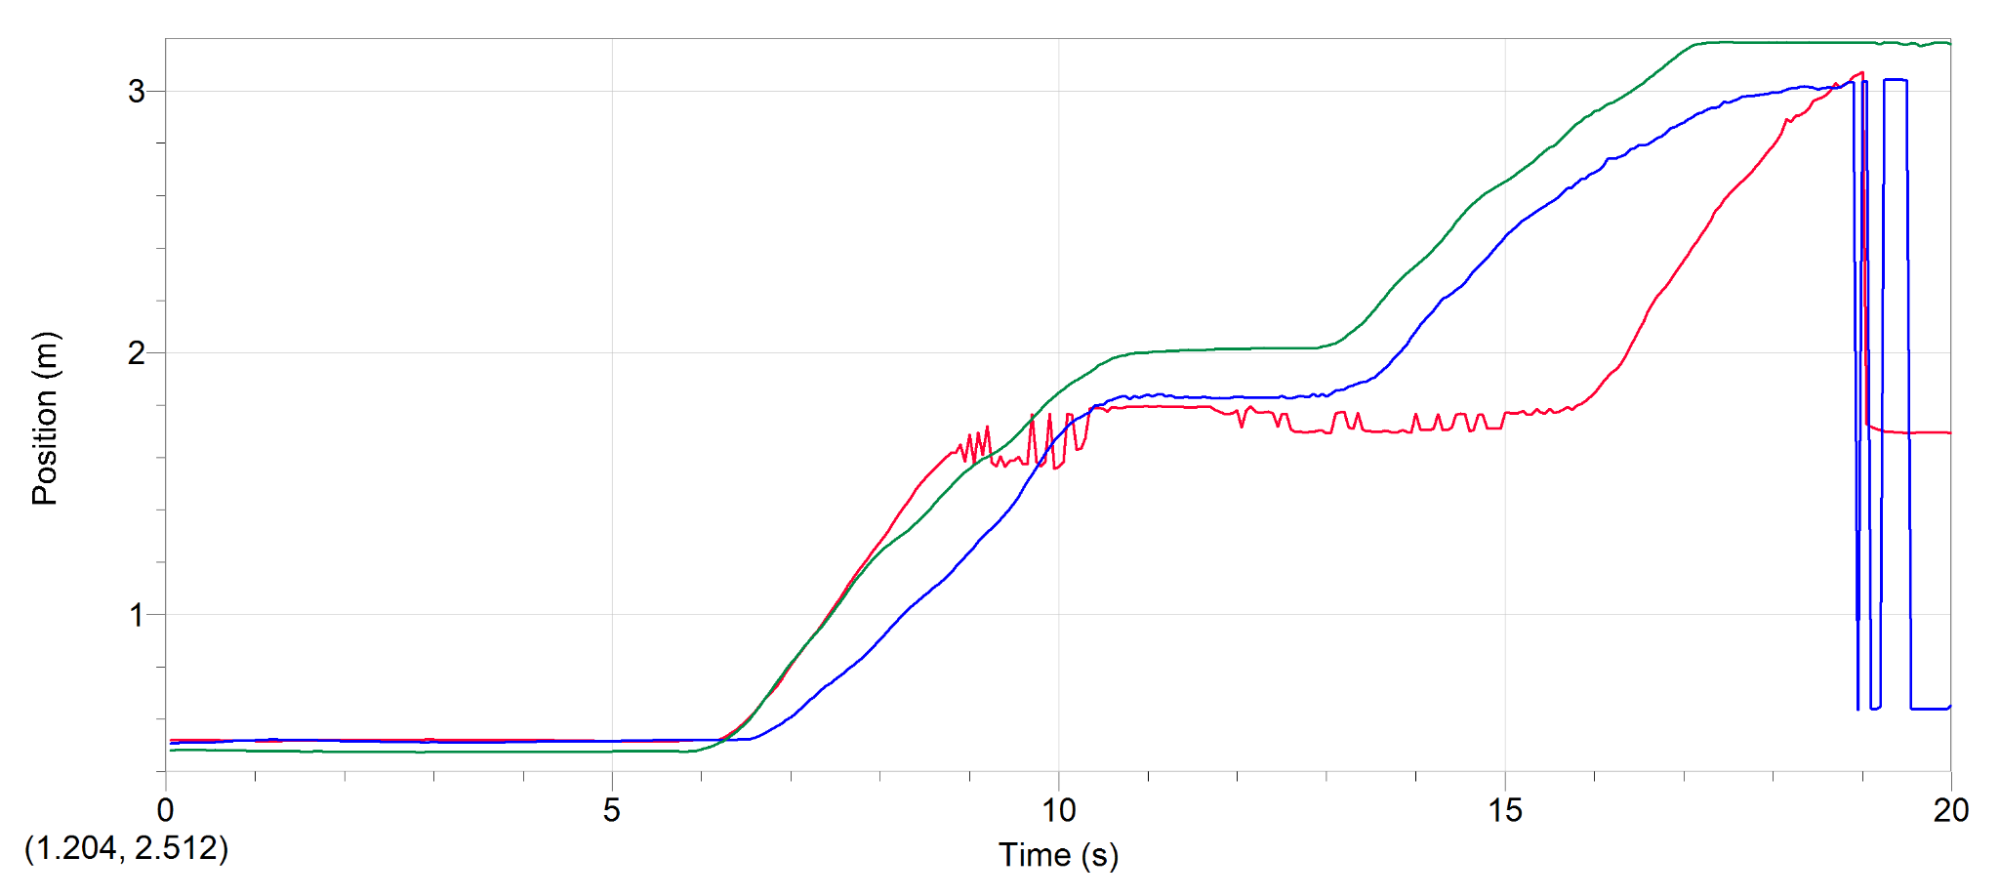
\includegraphics[width=0.8\textwidth]{image7.png}
    \end{mdframed}

    \subsection*{20.}

    \begin{mdframed}
        \centering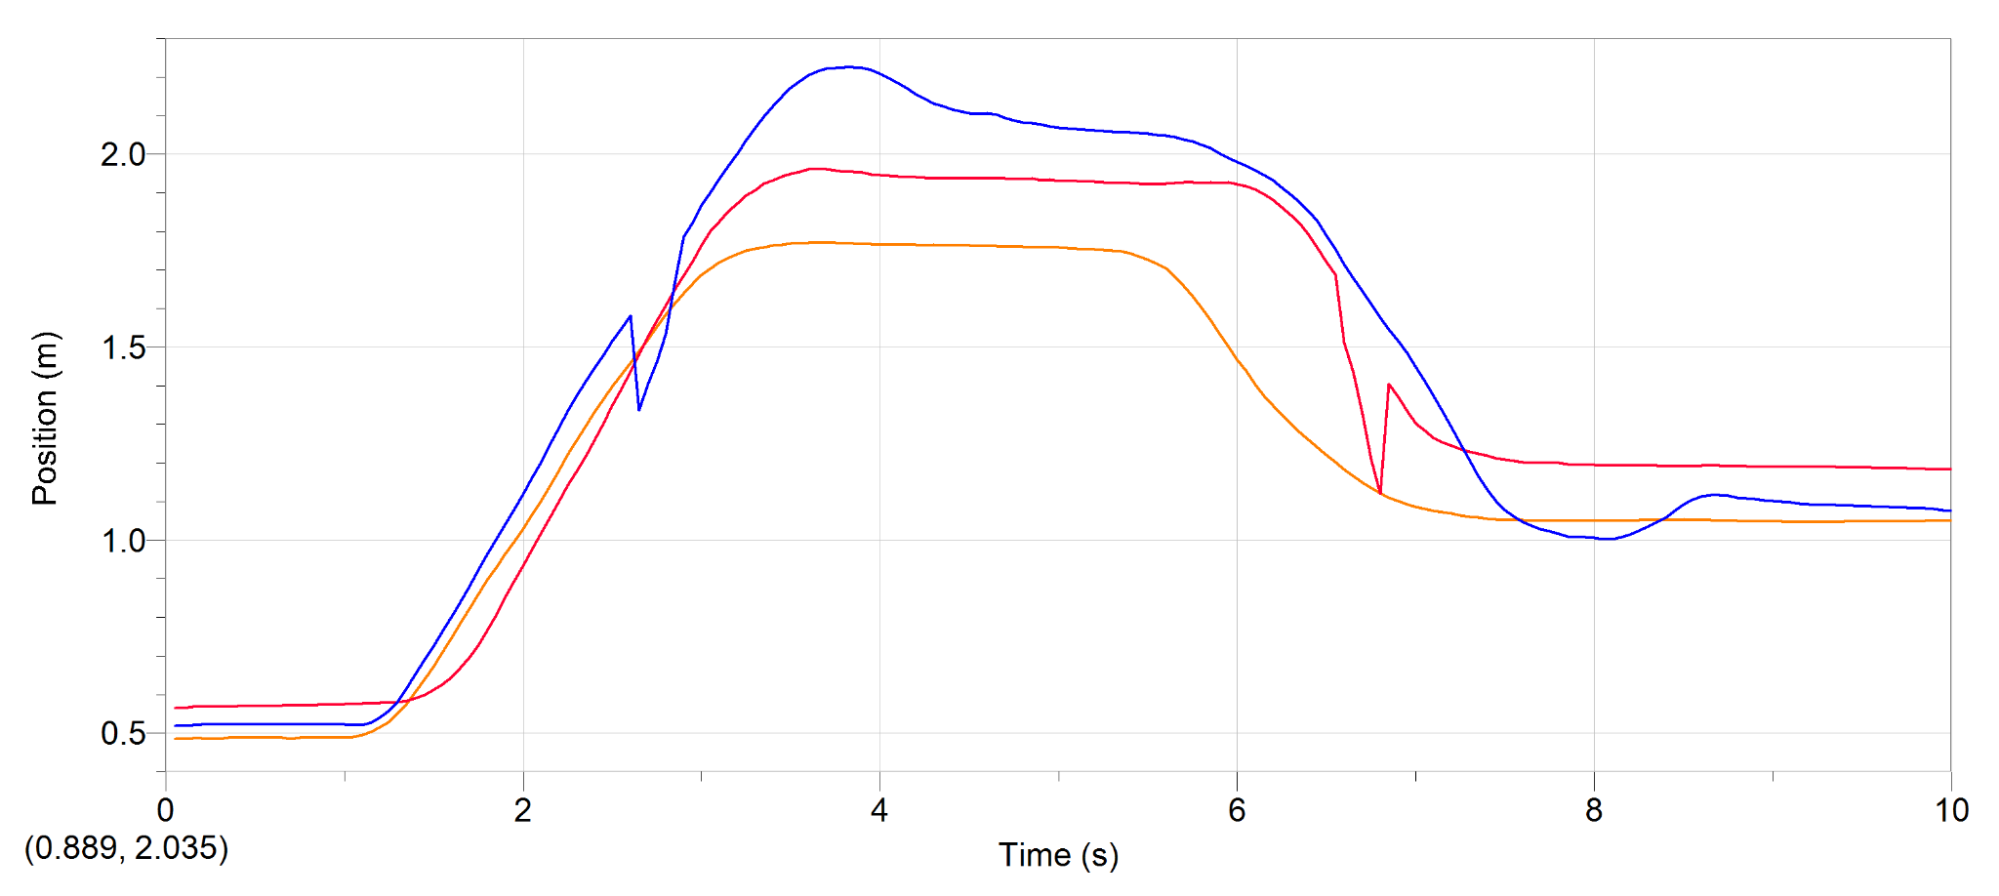
\includegraphics[width=0.8\textwidth]{image28.png}
    \end{mdframed}
    
    \subsection*{21.}

    \begin{mdframed}
        \centering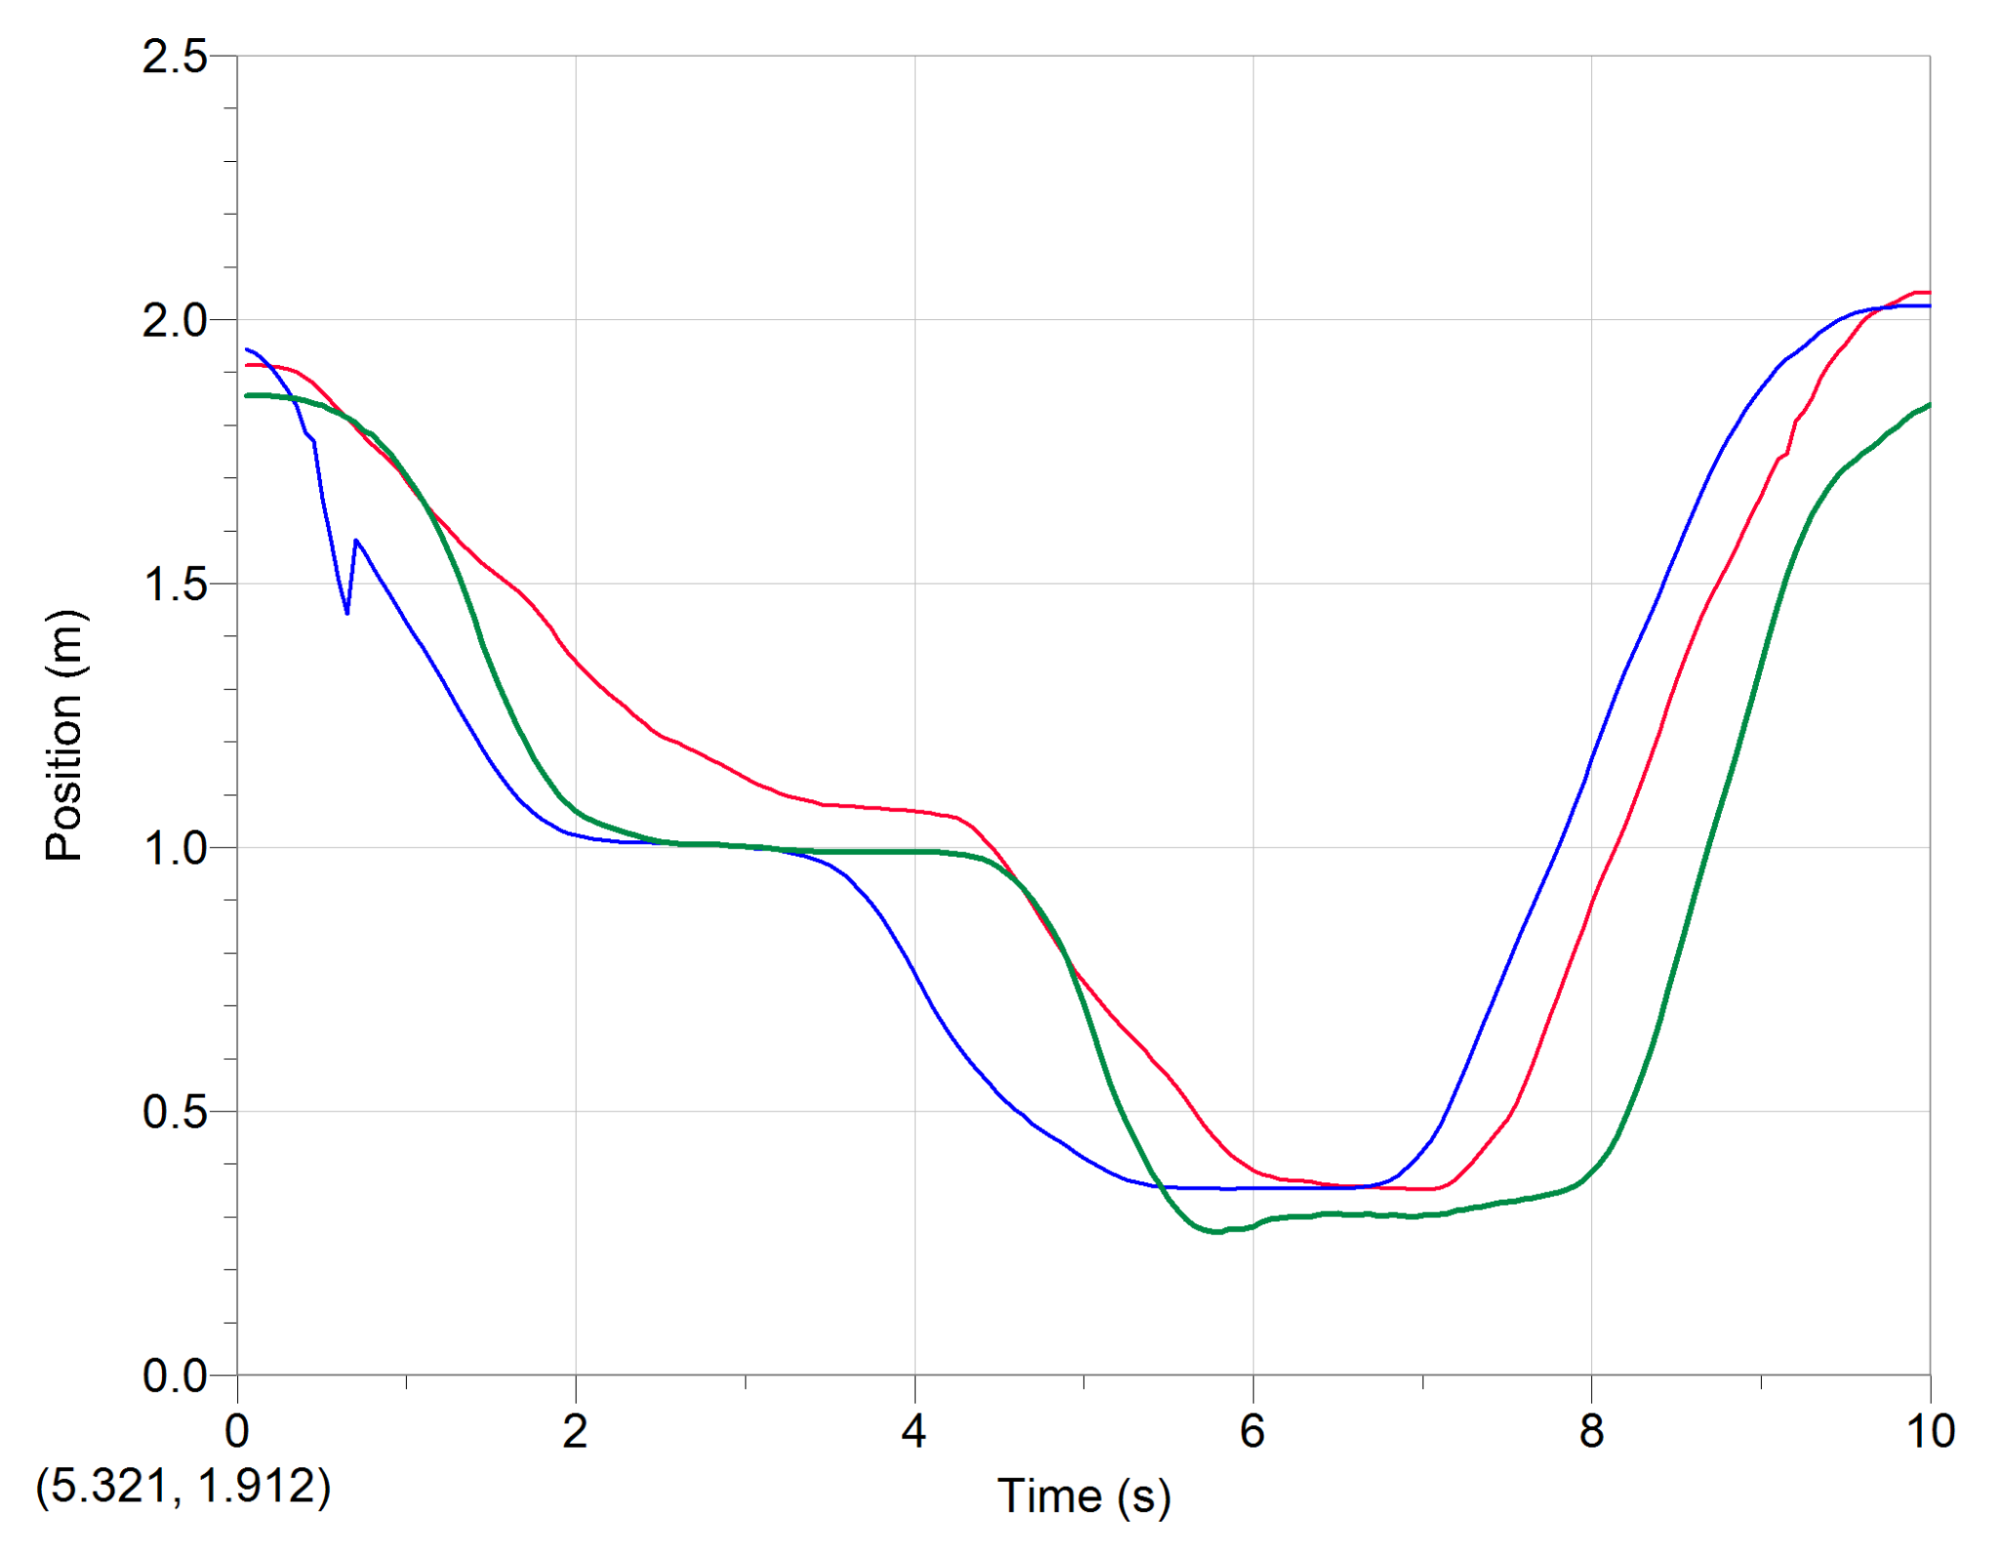
\includegraphics[width=0.8\textwidth]{image27.png}
    \end{mdframed}

    \subsection*{22.}

    \begin{mdframed}
        \centering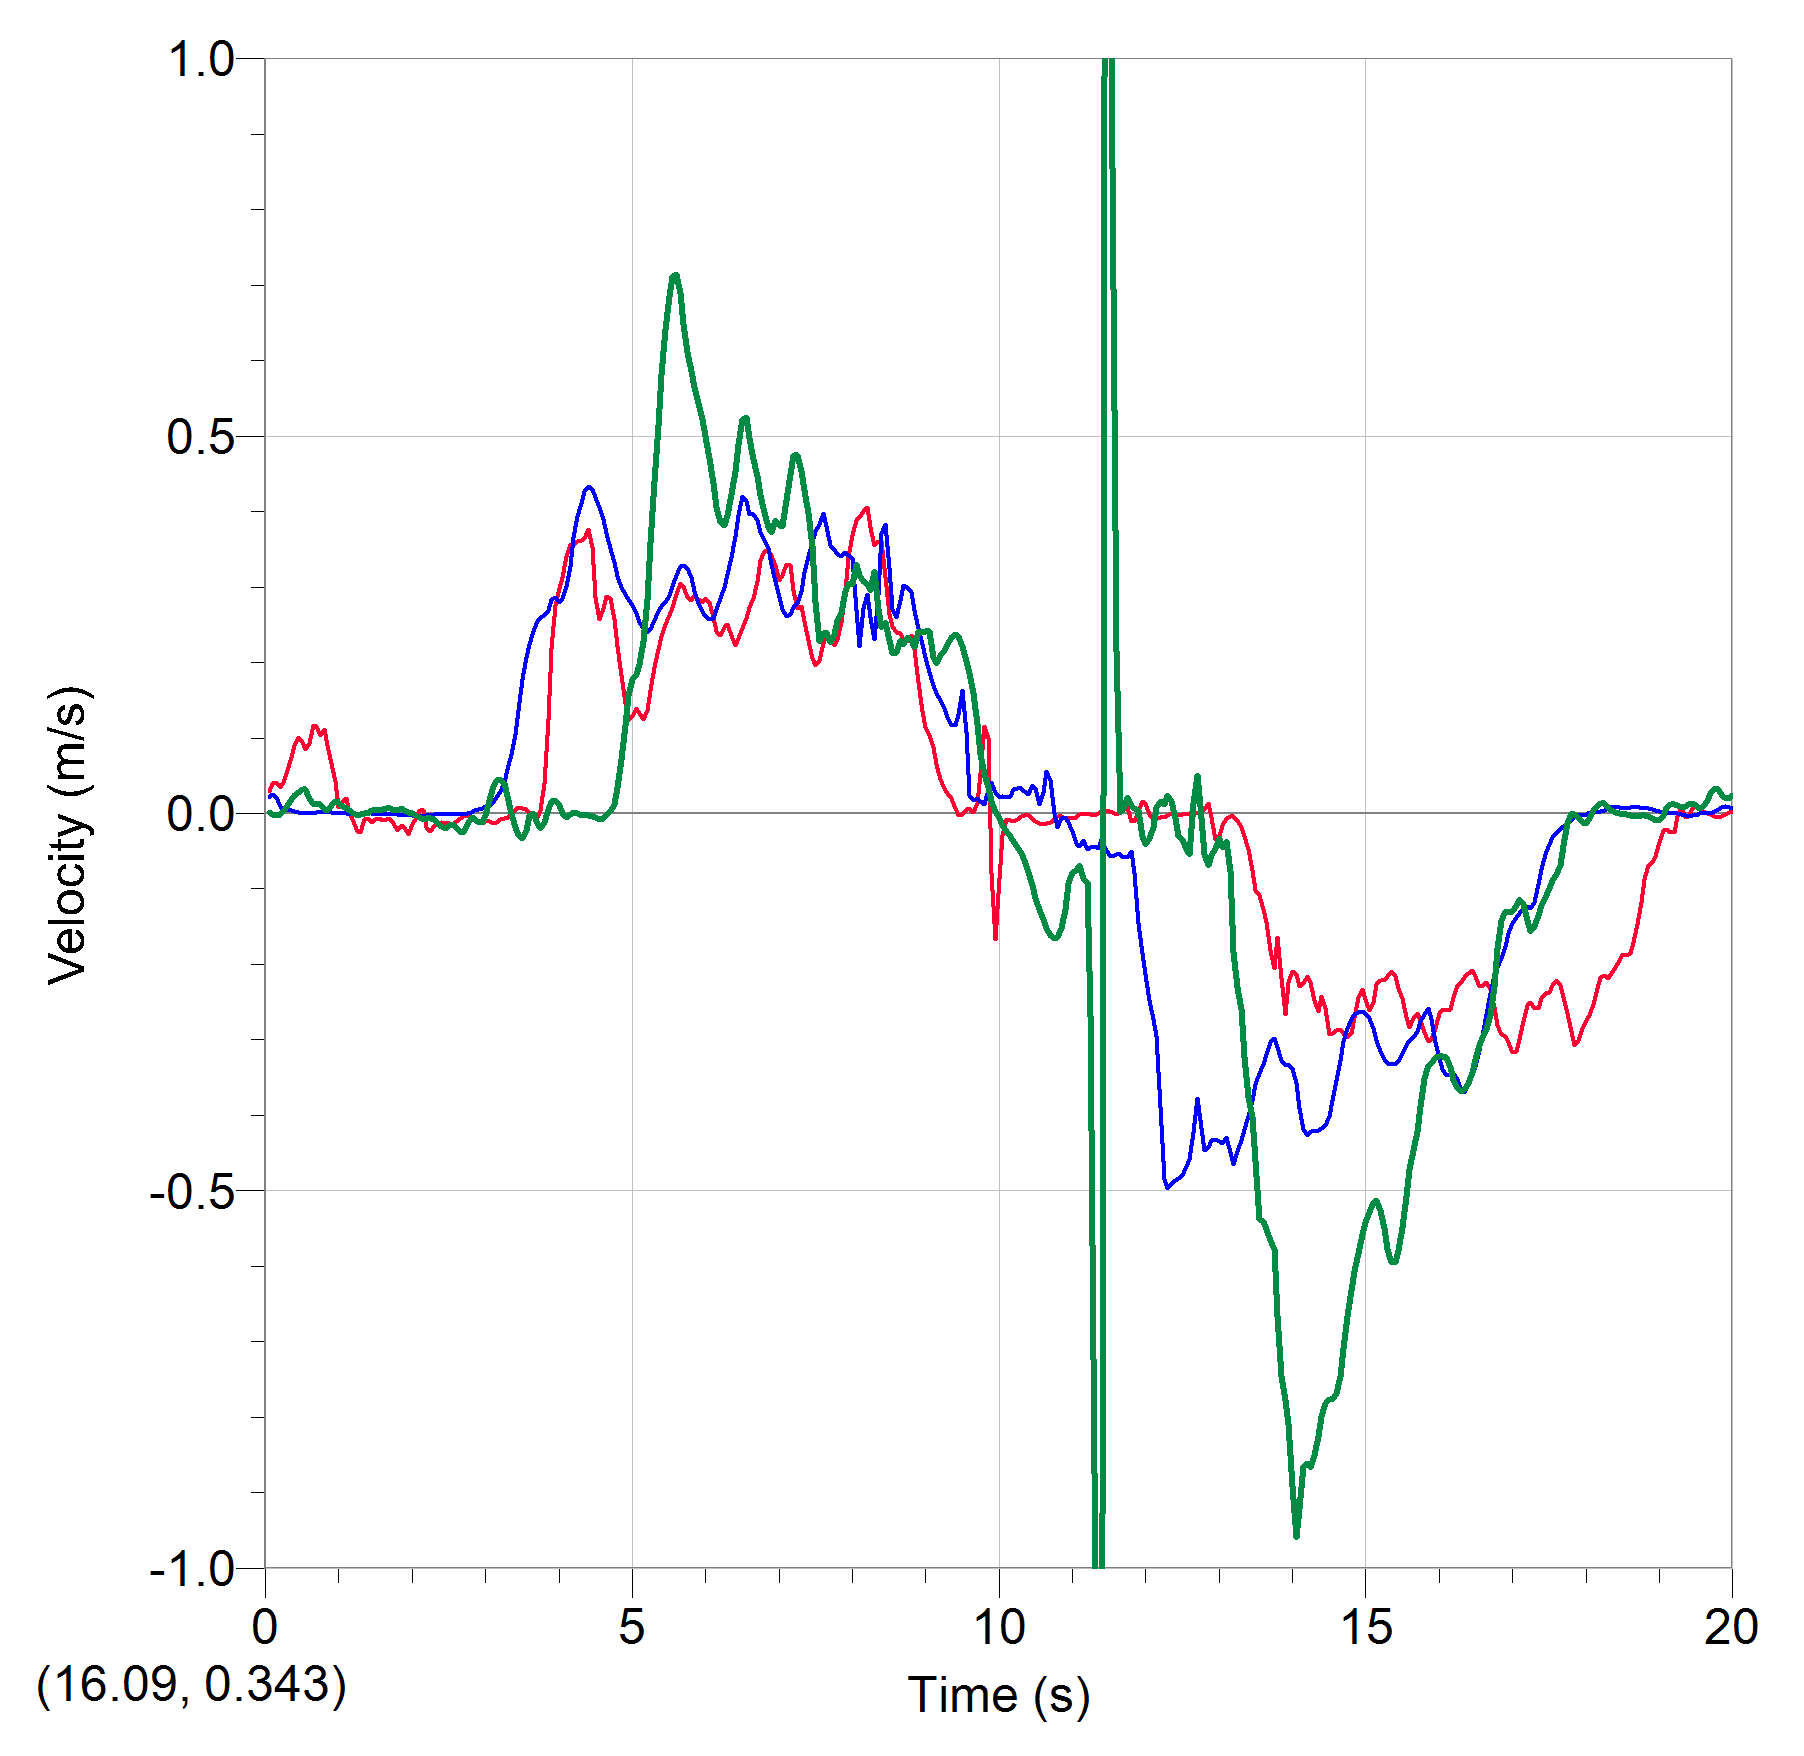
\includegraphics[width=0.8\textwidth]{image19.png}
    \end{mdframed}

    \subsection*{23.}

    \begin{mdframed}
        \centering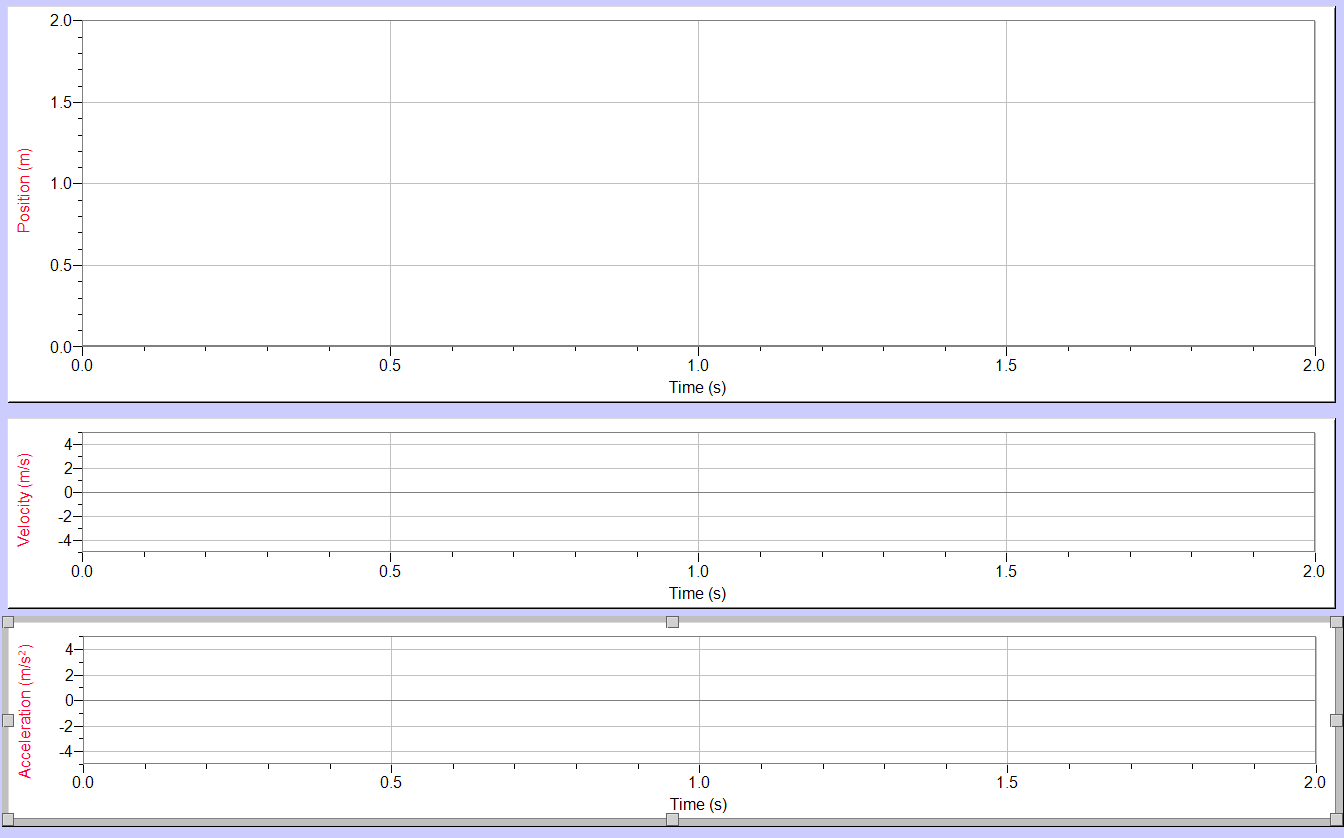
\includegraphics[width=0.8\textwidth]{image16.png}
    \end{mdframed}

    \pagebreak
    
    \subsection*{34.} 
    What information can and can’t be determined from a different plot? Please draw lines to match appropriately. To be thorough, you should write a few words on each line describing how one would obtain such information from that plot. For example, the initial position can be found from a position/time plot from something described as the “y-value”, “vertical value”, “height” or “value”:

    * There is a graph per plot.

    \begin{mdframed}
        \centering
        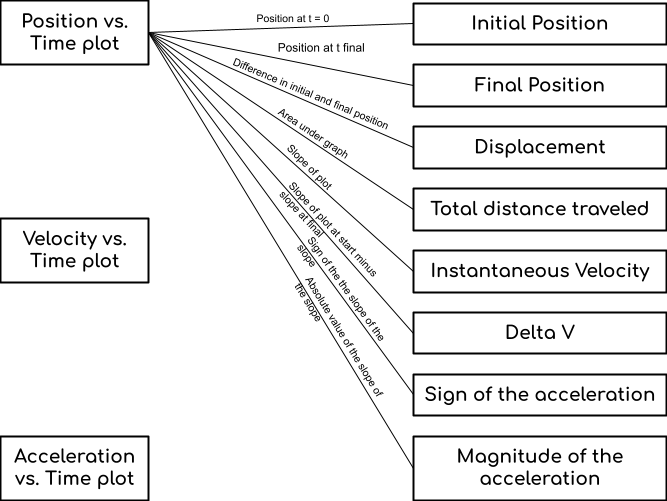
\includegraphics[width=0.8\textwidth]{image13.png}

        \horizontal

        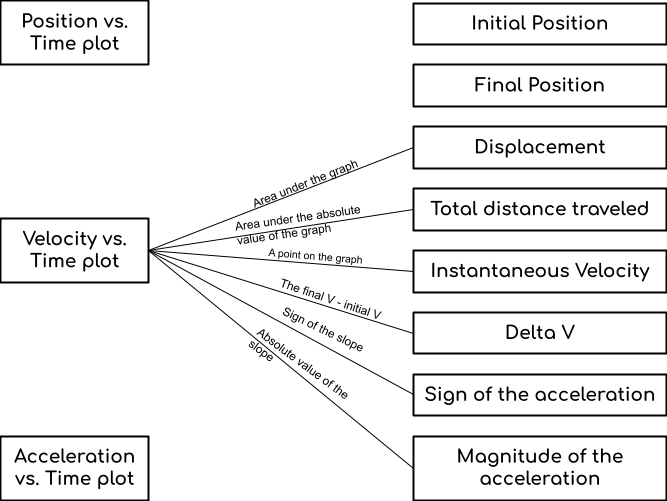
\includegraphics[width=0.8\textwidth]{image14.png}

        \horizontal

        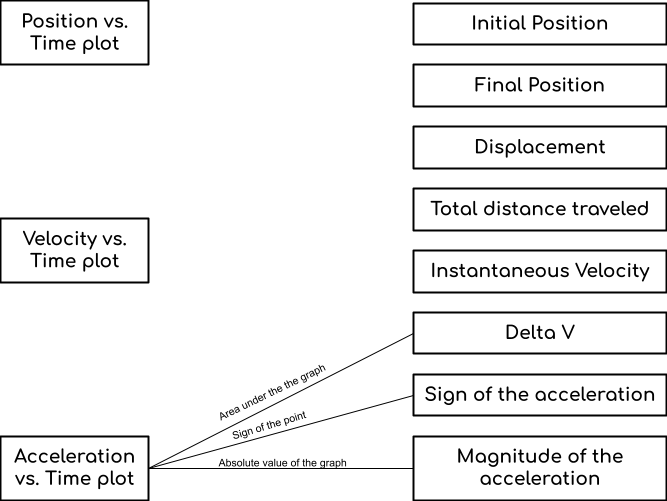
\includegraphics[width=0.8\textwidth]{image24.png}
    \end{mdframed}

\end{document}